\documentclass[tikz,border=8pt]{standalone}
% Shared look for every TikZ diagram. Load with \input{../../tools/tikz-style.tex}
\usepackage[T1]{fontenc}
\usepackage{lmodern}
\renewcommand{\sfdefault}{lmr}  % diagrams use the same serif as the text
\usetikzlibrary{arrows.meta, positioning, shapes.geometric, calc, fit, backgrounds}
\definecolor{cblue}{HTML}{4C78A8}
\definecolor{corange}{HTML}{F58518}
\definecolor{cgreen}{HTML}{54A24B}
\definecolor{cred}{HTML}{E45756}
\definecolor{cpurple}{HTML}{B279A2}
\definecolor{cgrey}{HTML}{6B6B6B}
\tikzset{
  every picture/.style={font=\sffamily, line width=1.2pt},
  box/.style={draw=#1, fill=#1!12, rounded corners=4pt, align=center, inner sep=7pt, minimum height=1.1cm},
  box/.default=cgrey,
  arrow/.style={-{Stealth[length=3mm]}, draw=cgrey, line width=1.4pt},
  title/.style={font=\sffamily\bfseries\Large},
  note/.style={font=\sffamily\small, text=cgrey, align=center},
}
\AtBeginDocument{\hyphenpenalty=10000 \exhyphenpenalty=10000}

\begin{document}
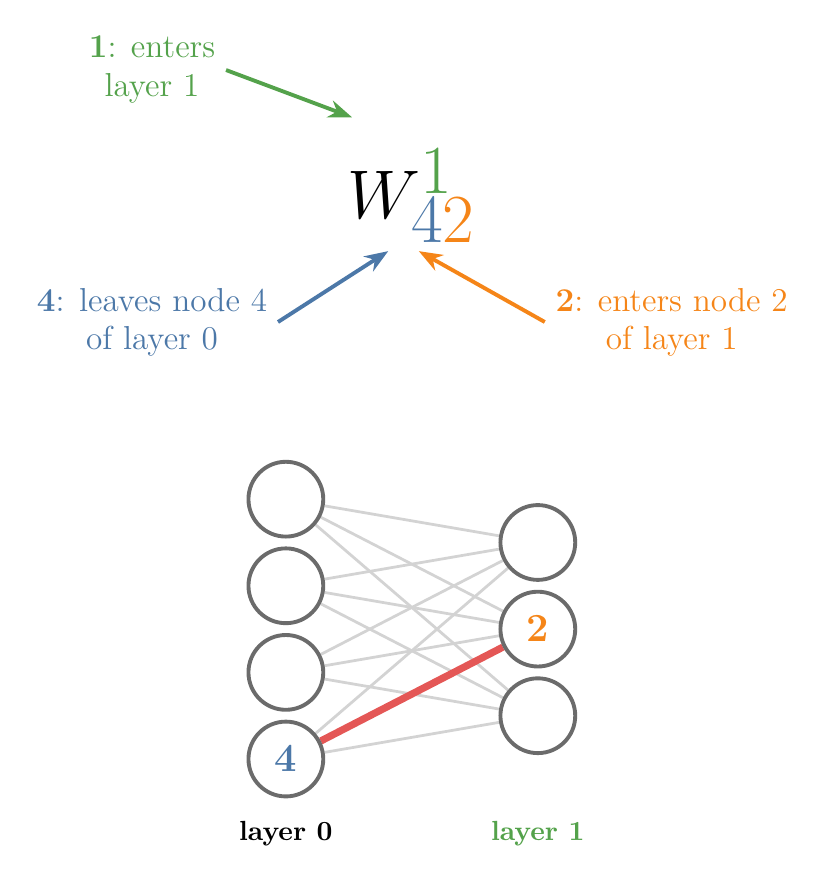
\begin{tikzpicture}[every node/.append style={font=\sffamily\large},
  inp/.style={circle, draw=cgrey, fill=white, minimum size=0.95cm, line width=1.4pt}]
  % symbol
  \node[font=\fontsize{40}{44}\selectfont] (W) at (0,0) {$W^{\textcolor{cgreen}{1}}_{\textcolor{cblue}{4}\textcolor{corange}{2}}$};
  \node[text=cgreen, align=center] (k) at (-3.3,1.6) {\textbf{1}: enters\\layer 1};
  \node[text=cblue, align=center] (i) at (-3.3,-1.6) {\textbf{4}: leaves node 4\\of layer 0};
  \node[text=corange, align=center] (j) at (3.3,-1.6) {\textbf{2}: enters node 2\\of layer 1};
  \draw[arrow, draw=cgreen] (k.east) -- ++(1.6,-0.6);
  \draw[arrow, draw=cblue] (i.east) -- ++(1.4,0.9);
  \draw[arrow, draw=corange] (j.west) -- ++(-1.6,0.9);
  % mini network
  \begin{scope}[shift={(-1.6,-5.0)}]
    \foreach \a in {1,...,4} \node[inp] (a\a) at (0, 2.25-1.1*\a) {};
    \foreach \b in {1,2,3} \node[inp] (b\b) at (3.2, 1.7-1.1*\b) {};
    \begin{scope}[on background layer]
    \foreach \a in {1,...,4} \foreach \b in {1,2,3} \draw[cgrey!30, line width=1pt] (a\a) -- (b\b);
    \draw[cred, line width=2.6pt] (a4) -- (b2);
    \end{scope}
    \node[cblue, font=\sffamily\bfseries\Large] at (a4) {4};
    \node[corange, font=\sffamily\bfseries\Large] at (b2) {2};
    \node[font=\sffamily\bfseries] at (0,-3.1) {layer 0};
    \node[font=\sffamily\bfseries, text=cgreen] at (3.2,-3.1) {layer 1};
  \end{scope}
\end{tikzpicture}
\end{document}
